\subsection*{Программный доступ к элементам презентации}
\addcontentsline{toc}{subsection}{Программный доступ к элементам презентации}

\textbf{Задание:}\\
По щелчку мыши строить в области просмотра фигуры различной формы.\\
Тип фигуры (КВАДРАТ, КРУГ, ОТРЕЗОК) определять с помощью радиокнопок, размер -- с помощью бегунка.\\
При нажатии кнопки 1 сформировать коллекцию кругов. Установить с помощью бегунка одинаковый радиус всех кругов.\\
По нажатию кнопки2 разместить их в ряд (строку) в нижней части области просмотра на равном расстоянии друг от друга.\\

\textbf{Решение:}\\
В начале создадим радио переключатель, в котором укажем все возможные типы объектов. Далее создадим бегунок, который будет определять размер фигуры.\\

Для того, чтобы фигуры создавались по щелчку мыши, необходимо создать прямоугольник размером с область просмотра, в котором следует  прописать какого типа и размера фигуру необходимо создать в месте клика мышки. (Рисунок \ref{fig:mouse1})

\begin{figure}[h]
	\centering 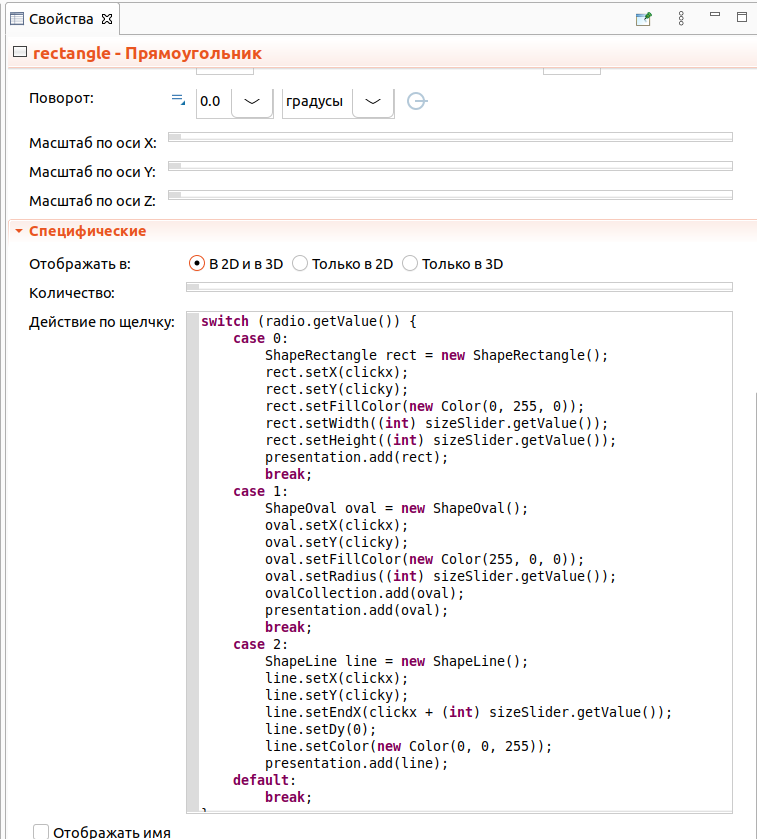
\includegraphics[scale=0.35]{mouse1}
	\caption{Алгоритм cоздания фигуры}
	\label{fig:mouse1}
\end{figure}

\newpage

При создании объекта типа <<круг>>, объект добавляется в коллекцию, в которой будут храниться все объекты этого типа. Теперь, когда все круги собраны в одной коллекции, необходимо создать кнопку, которая будет задавать кругам одинаковый размер. (Рисунок \ref{fig:mouse2})

\begin{figure}[h]
	\centering 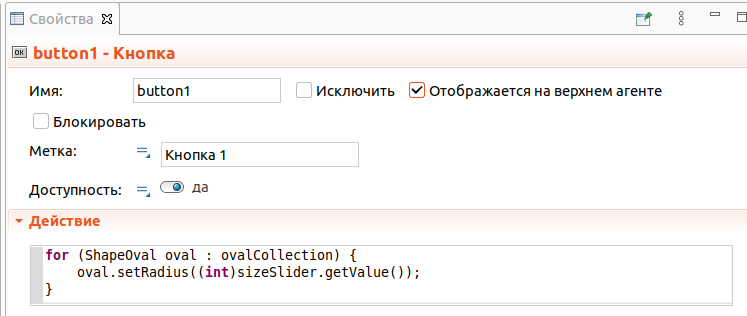
\includegraphics[scale=0.35]{mouse2}
	\caption{Задание одинаковых размеров}
	\label{fig:mouse2}
\end{figure}

Еще одним заданием было создание кнопки, которая размещает круги в ряд в нижней части области просмотра на равном расстоянии друг от друга относительно середины фигуры, расстояние задается при помощи бегунка. (Рисунок \ref{fig:mouse3})

\begin{figure}[h]
	\centering 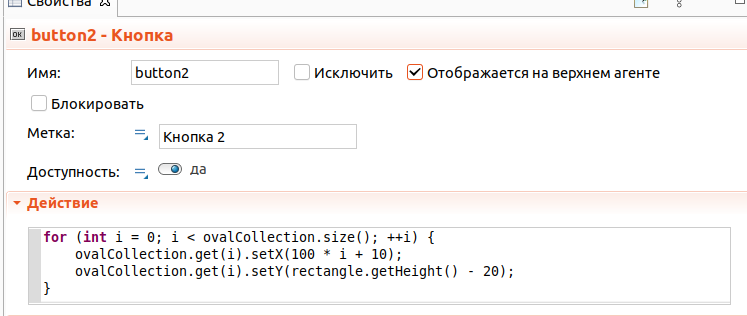
\includegraphics[scale=0.35]{mouse3}
	\caption{Размещение кругов в ряд}
	\label{fig:mouse3}
\end{figure}

\begin{figure}[h]
	\centering 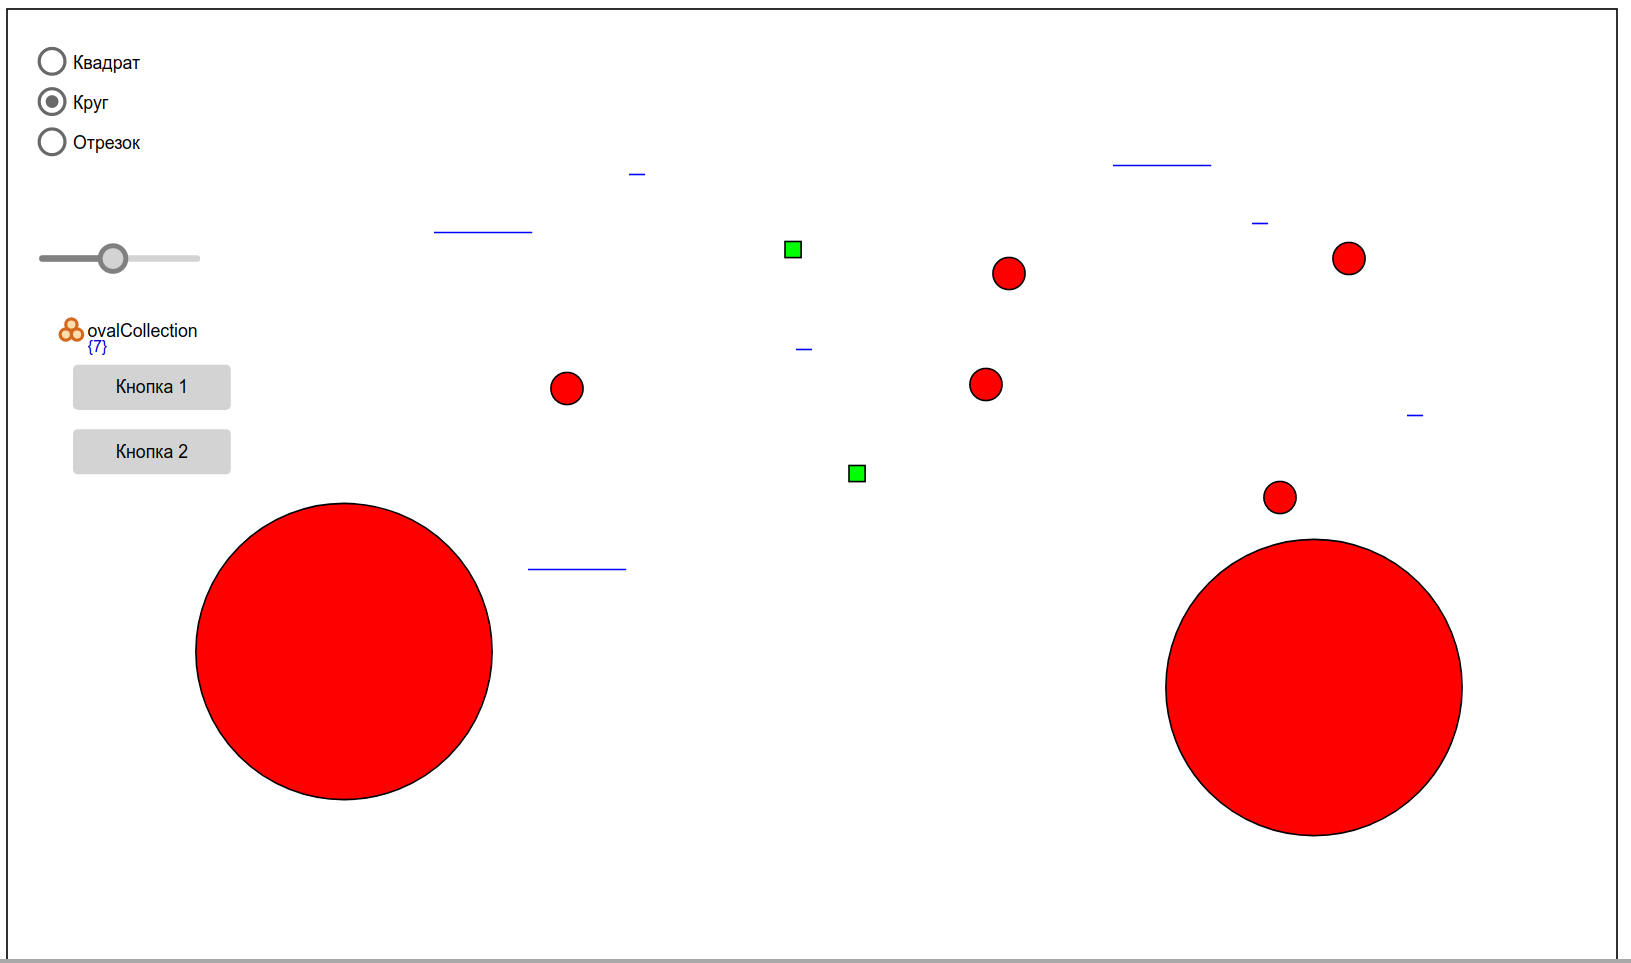
\includegraphics[scale=0.16]{mouse4}
	\caption{Визуализация работы получившейся модели}
	\label{fig:mouse4}
\end{figure}

Таким образом, нами был освоен механизм программного доступа к элементам презентации.\\